\documentclass[12pt, a4paper, twoside, openright, slovak]{book}

\usepackage[slovak]{babel}
\usepackage[utf8]{inputenc}
\usepackage[T1]{fontenc}
\usepackage[
	top=2.5cm,
	bottom=2.5cm,
	right=3.5cm,
	left=2.5cm
]{geometry}
%\usepackage{graphicx}
%\usepackage{hyperref}
%\usepackage{csquotes}
%\usepackage{listings}
%\usepackage{xcolor}
%\usepackage{enumitem}
%\usepackage{multirow}
%\usepackage{subcaption}
%\usepackage{fancyvrb}
\usepackage{setspace}
\usepackage{fancyhdr}
\usepackage{pdfpages}
\usepackage{amsmath}
\usepackage{tocloft}
\usepackage{csquotes}
\usepackage{expl3}
\usepackage[style=iso-numeric, backend=biber]{biblatex}
\addbibresource{literature.bib}
\AtBeginDocument{\renewcommand\appendixname{Príloha}}

\raggedbottom
\newcommand{\emptypage}{\newpage\thispagestyle{empty}\mbox{}\newpage}
\newcommand{\signaturespace}[2]{
  % #1 = width of the dotted line
  % #2 = legend
  \begingroup
  \renewcommand{\arraystretch}{0}
  \begin{tabular}[t]{cc}
  \hspace*{0pt}
  \cleaders\hbox{\kern.6pt.\kern.6pt}\hskip#1\relax
  \hspace*{0pt}
  \\[0.5cm]
  #2
  \end{tabular}
  \endgroup
}

\pagestyle{fancy}
\fancyhf{}  % clear all header and footers
\fancyhead[L]{\nouppercase{\leftmark}}
\fancyfoot[LE, RO]{\thepage}
\fancypagestyle{plain}{
  \fancyhf{}%
  \renewcommand{\headrulewidth}{0pt}%
  \fancyhf[lef,rof]{\thepage}%
}


\setstretch{1.5}
\newcommand{\University}[0] {Slovenská technická univerzita v Bratislave}
\newcommand{\UniversityEN}[0] {Slovak University of Technology Bratislava}
\newcommand{\Faculty}[0] {Fakulta informatiky a informačných technológií}
\newcommand{\FacultyEN}[0] {Faculty of Informatics and Information Technologies}
\newcommand{\Thesis}[0] {Bakalárska práca}
\newcommand{\ThesisEN}[0] {Bachelor's Thesis}
\newcommand{\Title}[0] {Spracovanie dát generovaných senzorovou IoT sieťou}
\newcommand{\TitleEN}[0] {Processing of Data Generated by the Sensor IoT Network}
\newcommand{\Author}[0] {Miroslav Hájek}
\newcommand{\Supervisor}[0] {Ing. Marcel Baláž, PhD.}
\newcommand{\PedagogicalSupervisor}[0] {Ing. Jakub Findura}
\newcommand{\RegNo}[0] {FIIT-1234-98765}
\newcommand{\Date}[0] {Máj 2022}
\newcommand{\DateEN}[0] {2022, May}
\newcommand{\StudyProgramme}[0] {Informatika}
\newcommand{\StudyProgrammeEN}[0] {Informatics}
\newcommand{\StudyField}[0] {Informatika}
\newcommand{\Institute}[0] {Ústav počítačového inžinierstva a aplikovanej informatiky, FIIT STU}
\newcommand{\SignPlace}[0] {V Bratislave, }
\newcommand{\SignDate}[0] {1.5.2022}


\begin{document}

% Obal
\thispagestyle{empty}
{\centering
	{\large \University}\par
	{\large \Faculty}\par
	\vspace{\medskipamount}
	\RegNo
	\vfill
	\textbf{\large \Author}\par
	\vspace{1.5\bigskipamount}
	\textbf{\Large \Title}\par
	\vspace{1.5\bigskipamount}
	{\large \Thesis}\par
	\vfill
}
\begin{flushleft}
Vedúci práce:\quad \Supervisor{\Large \par}
\vspace{\medskipamount}
\Date
\end{flushleft}

\emptypage

% Titulný list
\thispagestyle{empty}
{\centering
	{\large \University}\par
	{\large \Faculty}\par
	\vspace{\medskipamount}
	\RegNo
	\vfill
	\textbf{\large \Author}\par
	\vspace{1.5\bigskipamount}
	\textbf{\Large \Title}\par
	\vspace{1.5\bigskipamount}
	{\large \Thesis}\par
	\vfill
}
\begin{flushleft}
\begin{align*}
& \text{Študijný program:} && \text{\StudyProgramme} \\
& \text{Študijný odbor:} && \text{\StudyField} \\
& \text{Miesto vypracovania:} && \text{\Institute} \\
& \text{Vedúci práce:} && \text{\Supervisor} \\
& \text{Pedagogický vedúci:} && \text{\PedagogicalSupervisor}
\end{align*}
\vspace{2\bigskipamount}
\Date
\end{flushleft}

\emptypage

% Zadanie
\newpage
\thispagestyle{empty}
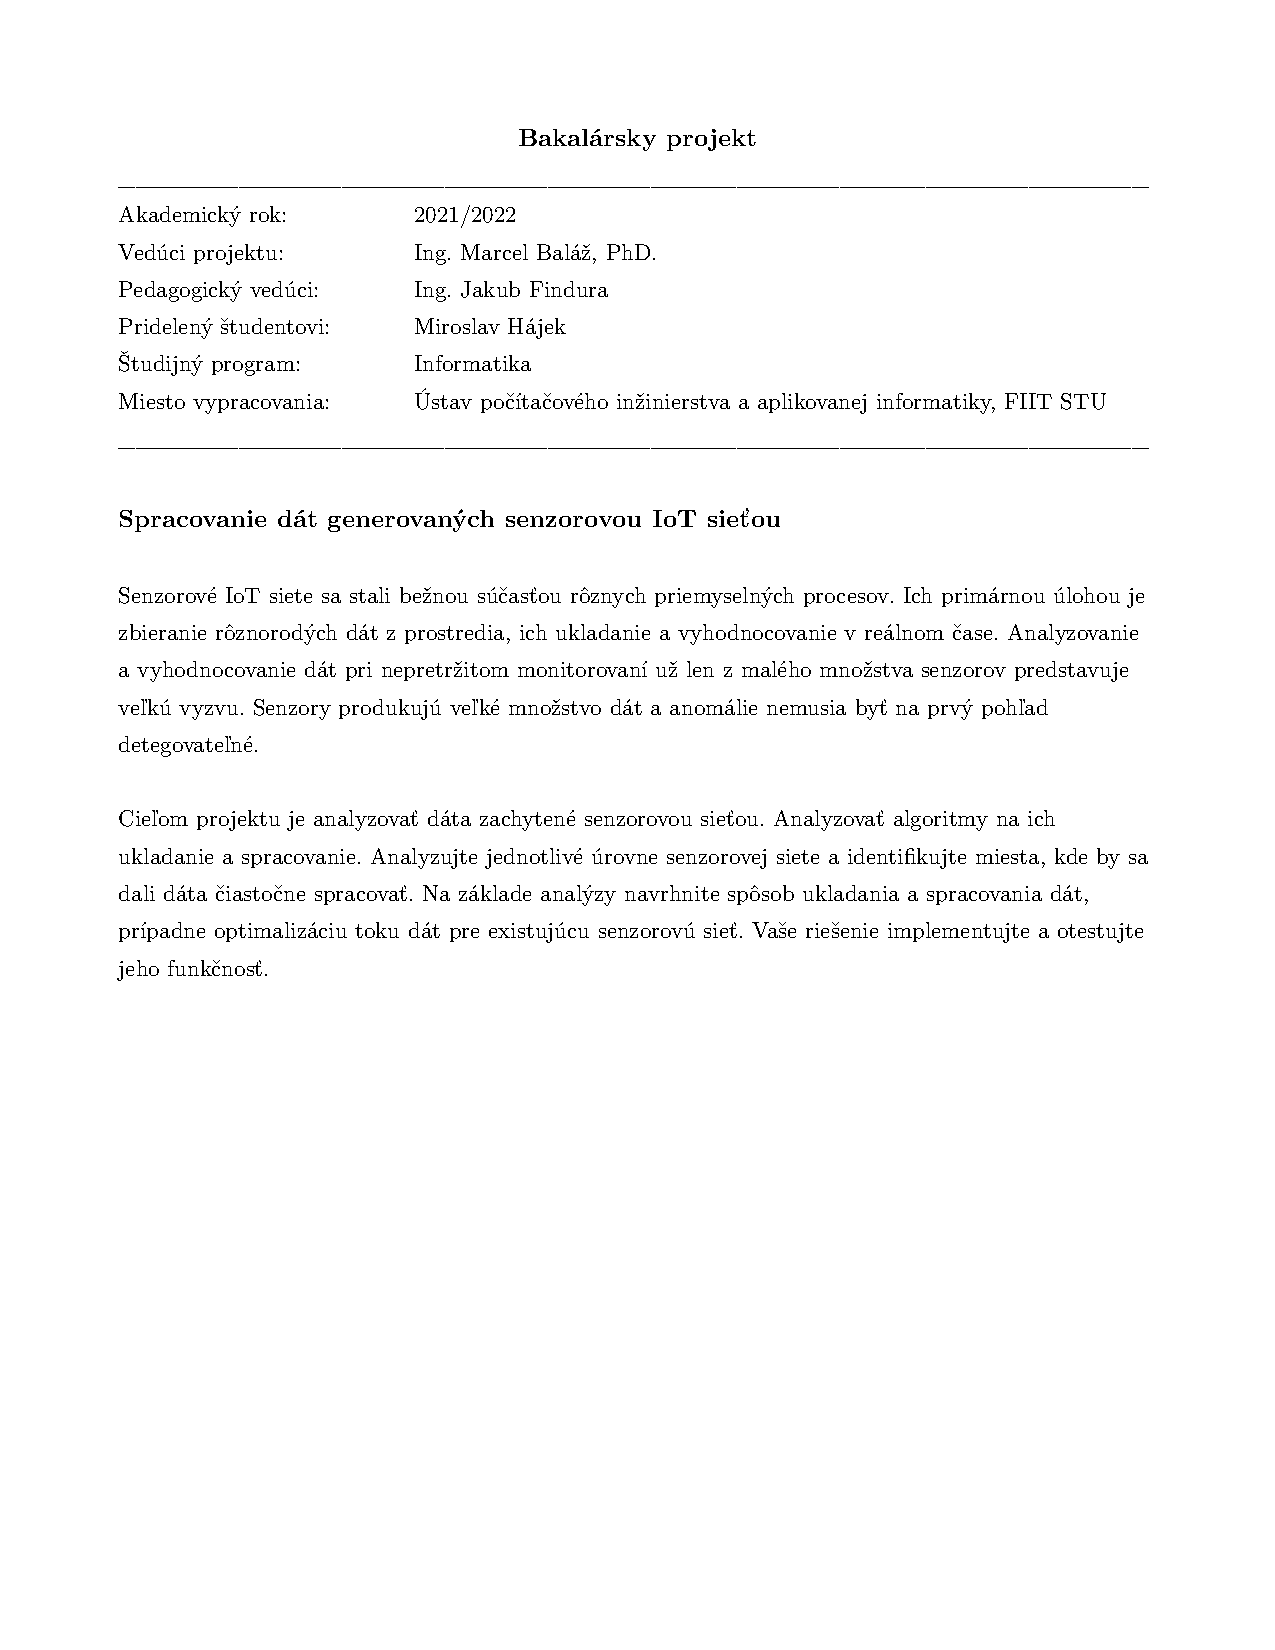
\includepdf[pages=1, scale=0.85]{zadanie}
\newpage

\emptypage
\pagenumbering{roman}

% Čestné prehlásenie
\thispagestyle{empty}
\vspace*{\fill}
\section*{Čestné prehlásenie}
Čestne vyhlasujem, že som túto prácu vypracoval samostatne, na základe konzultácií
a s použitím uvedenej literatúry.

\vspace{3\medskipamount}\noindent
\SignPlace \SignDate \hspace*{\fill} \signaturespace{5cm}{\Author}
\emptypage

% Poďakovanie
\thispagestyle{empty}
\vspace*{\fill}
\section*{Poďakovanie}
Text poďakovania
\emptypage

%Anotácia
\thispagestyle{empty}
\section*{Anotácia}
\University \\
\uppercase{\Faculty} \\
Študijný program: \text{\StudyProgramme}
\vspace{-8pt}
\begin{align*}
& \text{Autor:} && \text{\Author} \\
& \text{\Thesis:} && \text{\Title} \\
& \text{Vedúci bakalárskej projektu:} && \text{\Supervisor} \\
& \text{Pedagogický vedúci:} && \text{\PedagogicalSupervisor} \\
& \text{\Date}
\end{align*}
Stručná charakteristika zadania bakalárskeho projektu ale predovšetkým výsledkov bakalárskeho projektu v slovenskom a anglickom jazyku každá v rozsahu max. 1 strany A4 (hlavička + cca 150-200 slov).
\emptypage

%Anotácia EN
\thispagestyle{empty}
\section*{Annotation}
\UniversityEN \\
\uppercase{\FacultyEN} \\
Degree course: \text{\StudyProgrammeEN}
\vspace{-8pt}
\begin{align*}
& \text{Author:} && \text{\Author} \\
& \text{\ThesisEN:} && \text{\TitleEN} \\
& \text{Supervisor:} && \text{\Supervisor} \\
& \text{Departmental advisor:} && \text{\PedagogicalSupervisor} \\
& \text{\DateEN}
\end{align*}
Annotation text in English, 150-200 words.
\emptypage

% Obsah
\renewcommand{\contentsname}{Obsah}
\thispagestyle{empty}
\tableofcontents{}
\emptypage

% Kapitoly
\pagenumbering{arabic}

% include{chapter1}
\chapter{Úvod}
Záverečná správa (= finálny dokument bakalárskej práce) musí mať rozsah minimálne 20 normovaných strán (60 znakov na riadok, 30 riadkov na stranu). Toto platí pre hlavný obsah, teda obsah bez príloh a technickej dokumentácie.

Záverečná správa o riešení bakalárskeho projektu by mala obsahovať súčasti uvedené nižšie. Presné pokynu sú súčasťou zadania bakalárskeho projektu, konzultujte s vedúcim bakalárskeho projektu.

Obsahové (aj formálne) požiadavky na priebežnú správu k riešeniu bakalárskeho projektu odovzdávané v rámci BP I sú stanovené rovnako po konzultácii s vedúcim bakalárskeho projektu a spravidla sú podmnožinou požiadaviek na záverečnú správu).

\emptypage
\chapter{Analýza}
Táto časť bakalárskeho projektu má:

\begin{itemize}
\item poskytovať obraz o stave riešenia daného problému známeho z preštudovanej literatúry (nielen informácie z prednášok, prípadne skrípt a katalógov),
\item  porovnanie podobných riešení, ich kategorizáciu s uvedením charakteristických atribútov atď., podľa charakteru bakalárskeho projektu
\item  zdôvodnenie voľby spôsobu riešenia a stručný opis celkového spôsobu riešenia (napr. v opise sa treba sústrediť na prípadné modifikácie použitých štandardných metodík a ich zdôvodnenie z hľadiska splnenia cieľov projektu)
\end{itemize}

\section{Podsekcia}
Text
\emptypage


\chapter{Opis riešenia}
Táto časť bakalárskeho projektu obsahuje opis výsledkov riešenia jednotlivých etáp projektu. V prípade, že záverečný projekt nerieši všetky etapy, malo by byť v príslušnej časti uvedené kto, resp. kde sa príslušná etapa rieši/riešila/bude riešiť.

Typické etapy riešenia pri tvorbe softvérového systému:
\begin{itemize}
    \item špecifikácia požiadaviek
    \item návrh
    \item implementácia (ak to zadanie požaduje)
    \item overenie riešenia
\end{itemize}

Podľa možností treba vychádzať zo známych prístupov (napr. pri softvérových projektoch štruktúrovaný alebo objektovo orientovaný prístup) a techník (napr. blokové schémy, vývojové diagramy, UML, entito-relačné diagramy atď.). Táto časť práce závisí od konkrétneho zadania.
Je dôležité prezentovať návrhové rozhodnutia, alternatívy, ktoré sa zvažovali pri riešení a samotný návrh riešenia zadaného problému. Štruktúrovanie textu tejto časti DP by malo vychádzať zo zadanej úlohy, ktorá sa rieši. Najmä v tejto časti študent preukazuje tvorivý prístup k riešeniu problémov a kritické myslenie.
\emptypage


\chapter{Zhodnotenie}
Hlavné výsledky práce, prípadne porovnanie s inými prístupmi, možné smery ďalšieho rozvíjania.
Tu sa musí presne špecifikovať, čo je pôvodné a čo riešiteľ prebral.
\emptypage


\pagenumbering{gobble}
\nocite{*}
\printbibliography[title={Literatúra}]
%\emptypage

% no page numbers for appendicies
\addtocontents{toc}{\protect\setcounter{tocdepth}{0}}
\addtocontents{toc}{\cftpagenumbersoff{chapter}}
\appendix

% Príloha
\setcounter{figure}{0}
%\setcounter{listing}{0}
\chapter{Technická dokumentácia}
\pagenumbering{arabic}
\renewcommand*{\thepage}{A-\arabic{page}}

Prílohy dopĺňajú hlavnú časť práce. Obsahujú napríklad podrobné informácie k jednotlivým
etapám riešenia projektu. Typicky sa tu uvádza aj podstatná časť technickej dokumentácie.
Pozor, prílohy nesmú obsahovať také informácie, ktoré sú pre pochopenie práce kľúčové. Tie
musí obsahovať hlavná časť práce, ktorá musí byť úplná, celistvá.

Súčasťou príloh nie je len textový obsah, ale aj ďalšie artefakty, ktoré sú výsledkom projektu,
napr. počítačový kód, dátové vzorky, vedecký článok či plagát. Zvláštnu pozornosť venujte tým
artefaktom, ktoré sú potrebné pre replikovateľnosť postupov opisovaných v práci (napr. aby
mohol oponent pri vyhodnocovaní práce zopakovať uvádzané postupy a prísť k rovnakým
záverom). 

Digitálne artefakty sa prikladajú na elektronickom médiu. K akémukoľvek
digitálnemu obsahu treba uviesť v dokumente priebežnej či záverečnej správy
bakalárskej/diplomovej práce primeraný textový opis, preto nezabudnite digitálne médium
zdokumentovať. Prinajmenšom medzi prílohy zaraďte kapitolu „Obsah elektronického média“.
Na prílohy sa nezabudnite z hlavnej časti práce primerane odkazovať.

Obsah technickej dokumentácie závisí od povahy riešeného problému. Uvádza sa technická dokumentácia k systému (počítačový, softvérový), ktorý bol vytvorený v rámci riešenia projektu (ak sa toto v zadaní požadovalo). Samotný obsah a rozsah závisí aj od účelu vytvoreného systému (produkt, experimentovanie a pod.)
V prípade softvérového systému technická dokumentácia spravidla obsahuje časti v náväznosti na etapy tvorby softvérového systému:
\begin{itemize}
	\item dokumentáciu k etape špecifikácie požiadaviek
    \item dokumentáciu k etape návrhu projektu
    \item dokumentáciu k implementácii
    \item v prípade, že súčasťou riešenia sú programy, dokumentáciu k implementácii tvoria zdrojové texty programov
    \item v prípade, že súčasťou riešenia je návrh zariadenia, dokumentáciu k implementácii tvorí technická dokumentácia (schémy zapojenia, návrh dosiek plošných spojov, schémy rozmiestnenia súčiastok, zoznam použitých súčiastok, opis konektorov atď.)
    \item dokumentáciu k overeniu riešenia
    \item dokumentáciu k používaniu a údržbe (návody na použitie a údržbu projektu)
\end{itemize}


% Harmonogram práce
\thispagestyle{empty}
\chapter{Harmonogram práce}
\pagenumbering{arabic}
\renewcommand*{\thepage}{B-\arabic{page}}
\section{Zimný semester}
\section{Letný semester}

% Digitálne médium
\thispagestyle{empty}

\chapter{Obsah digitálneho média}
\pagenumbering{arabic}
\renewcommand*{\thepage}{C-\arabic{page}}
\par Evidenčné číslo práce v informačnom systéme: \RegNo
\par Obsah digitálnej časti práce (archív ZIP):
\par Názov odovzdaného archívu: ...zip

\end{document}